\providecommand{\main}{../../../..}
\documentclass[\main/dresen_thesis.tex]{subfiles}
\begin{document}
  \label{sec:looselyPackedNS:nanoparticle:sas}
  Small-angle X-ray scattering measured at GALAXI (\refch{ch:lss:galaxi}) and small-angle neutron scattering measured at D33 (\refch{ch:lss:d33}) was performed to quantitatively characterize the nanoparticle dispersions.
  The azimuthally averaged data is shown in \reffig{fig:looselyPackedNP:nanoparticle:sas}.
  From the qualitative comparison of the data, it is visible that the first form factor minima appears for IOS-11 at smaller $q$ values than for IOS-7 and that the minima of IOS-11 are sharper.
  The smaller $q$ value of the scattering vector translates to a larger particle size and the sharper minima to a smaller size distribution.
  Both observations are in agreement with the observations from TEM (\refsec{sec:looselyPackedNS:nanoparticle:tem}).

  \paragraphNewLine{Determination of Particle Sizes And Core-Shell Structure with SAS}

    To determine the size of the particles, the data for both samples and both experiments is fitted to a form factor of spherical core-shell particles with an additional oleic acid surfactant shell dispersed in cyclohexane.
    The best fit is shown in \reffig{fig:looselyPackedNP:nanoparticle:sas}, where the scattering length density profile is in each case shown in the insets.
    In all cases, the SLD of the core is fixed to the value of w\"ustite and the shell to magnetite.
    Furthermore the SLD of oleic acid and the solvents, cyclohexane for SAXS and toluene-$\mathit{d8}$ for SANS respectively, are fixed.
    The parameters of the two form factors are given in \reftab{tab:looselyPackedNP:nanoparticle:sas}.

    For IOS-11 the spherical core-shell-surfactant form factor shows a small deviation for small $q$ values.
    This is caused by a too high particle concentration in the dispersion, which results in a structure factor for small $q$.
    For larger $q$ values the structure factor is however negligible and therefore the data can still be well described by the form factor.
    For both SAXS and SANS a total particle diameter of $10.8 \unit{nm}$ is used, where for SANS a larger shell thickness for the magnetite phase of $1.6 \unit{nm}$ is needed in comparison to the value of $0.46 \unit{nm}$ obtained from SAXS.
    For the SANS measurement, the nanospheres were dried over night for redispersion in toluene-$\mathit{d8}$, therefore it is conceivable that they oxidized stronger in comparison to the SAXS measurement during that time.
    It is noteworthy that otherwise the SAXS and SANS experiment have been performed within the same week.

    For IOS-7, the size of the w\"ustite core has to be set to zero to properly describe the experimental SAS data by the spherical core-shell-surfactant form factor.
    Also, it is necessary to assume a bimodal distribution of particles.
    The obtained particle diameter is $7.08 \unit{nm}$ with a size distribution of $7.5 \unit{\%}$ for the first mode and $1.36 \unit{nm}$ with a size distribution of $60 \unit{\%}$, where the second mode makes up $78 \unit{\%}$ of the dispersion.

    \begin{figure}[!htbp]
      \centering
      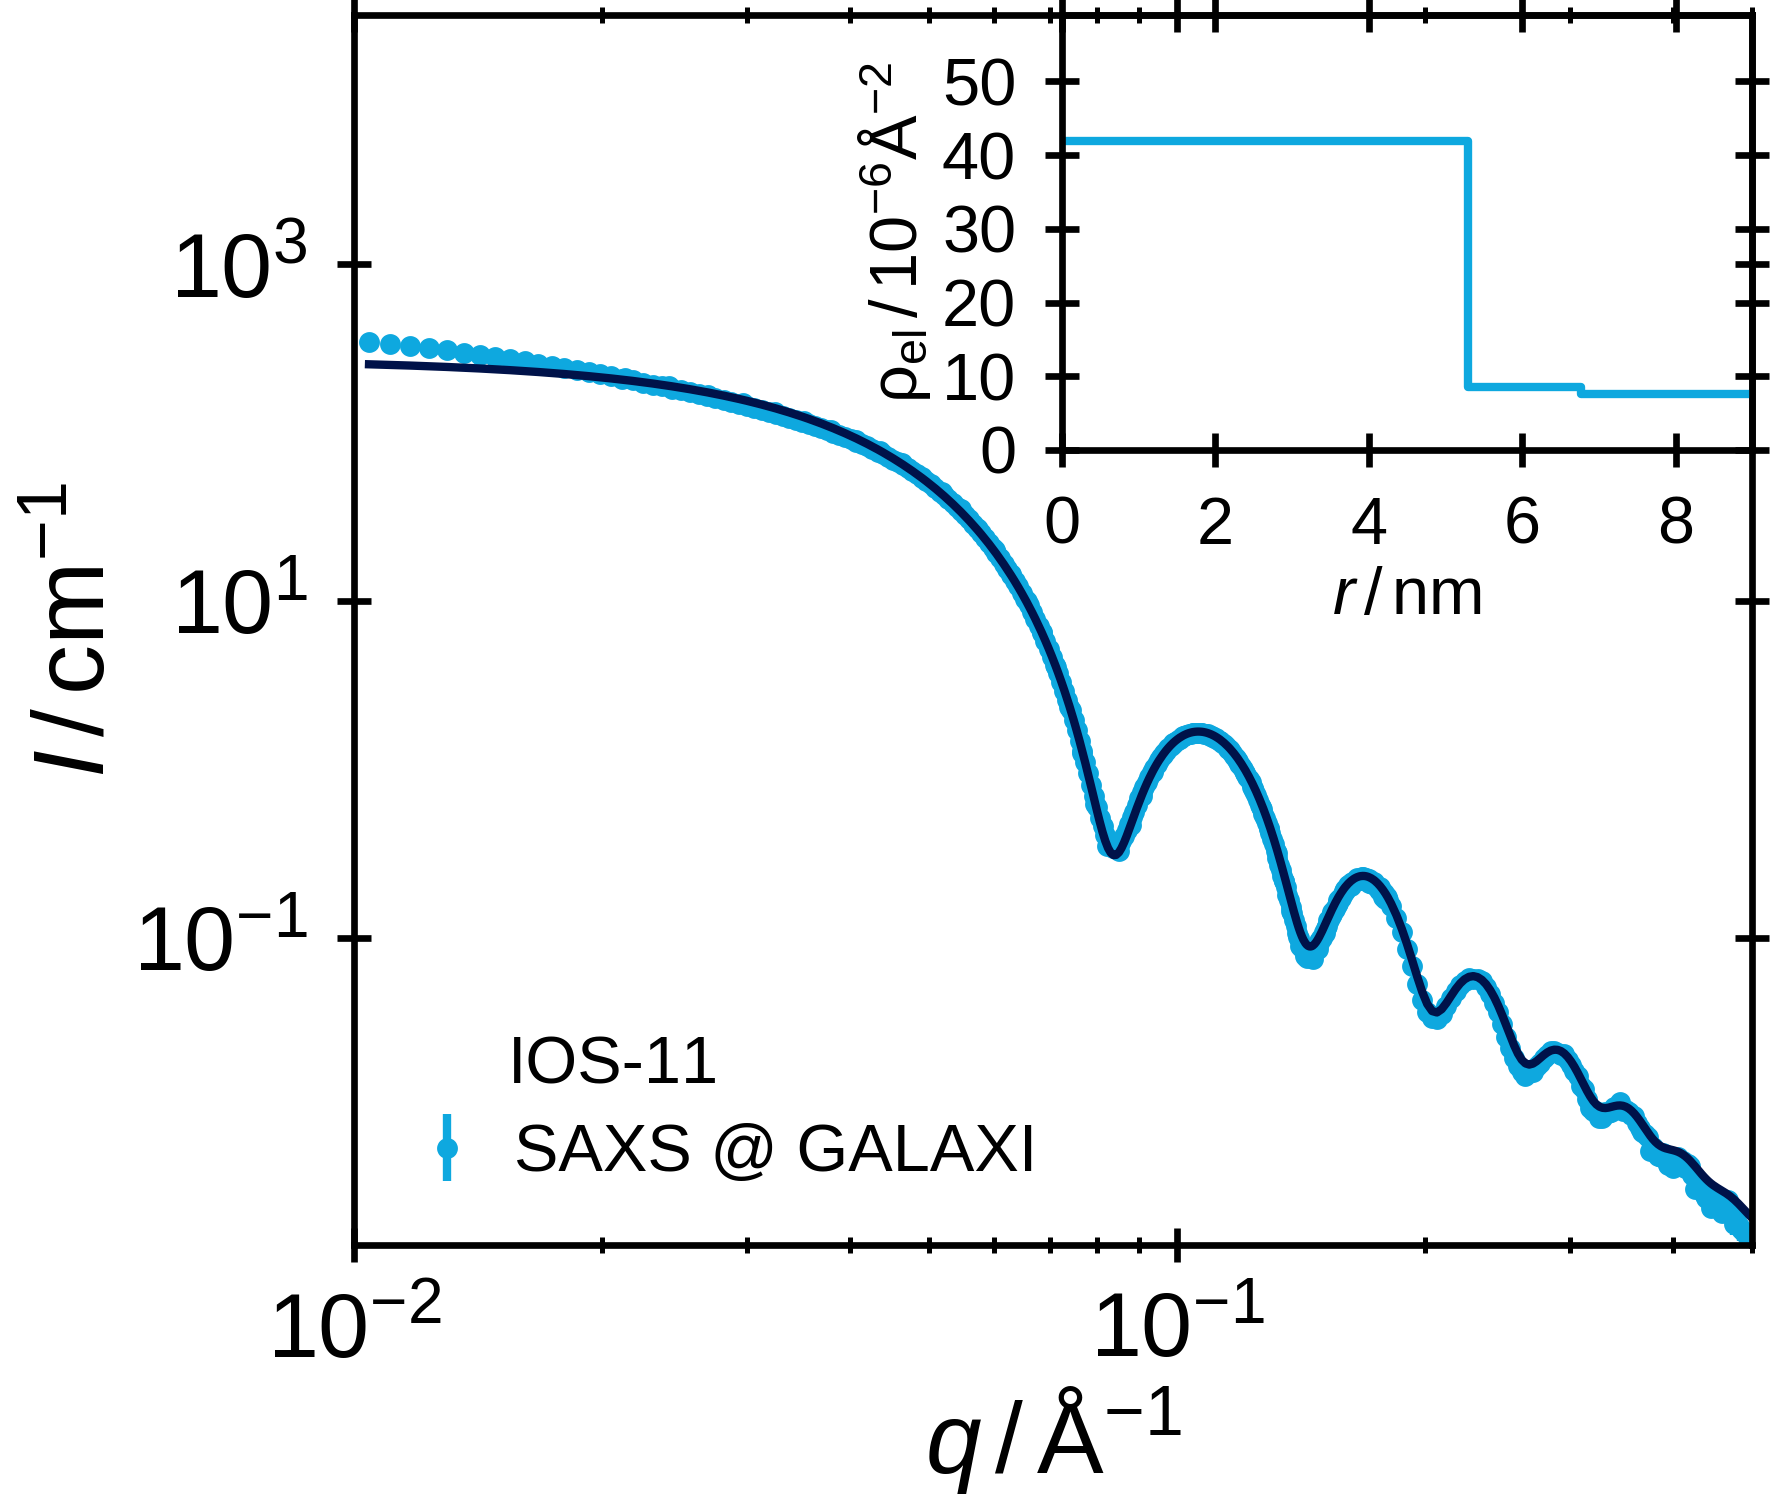
\includegraphics{looselyPackedNP_SAS_IOS-11_SAXS}
      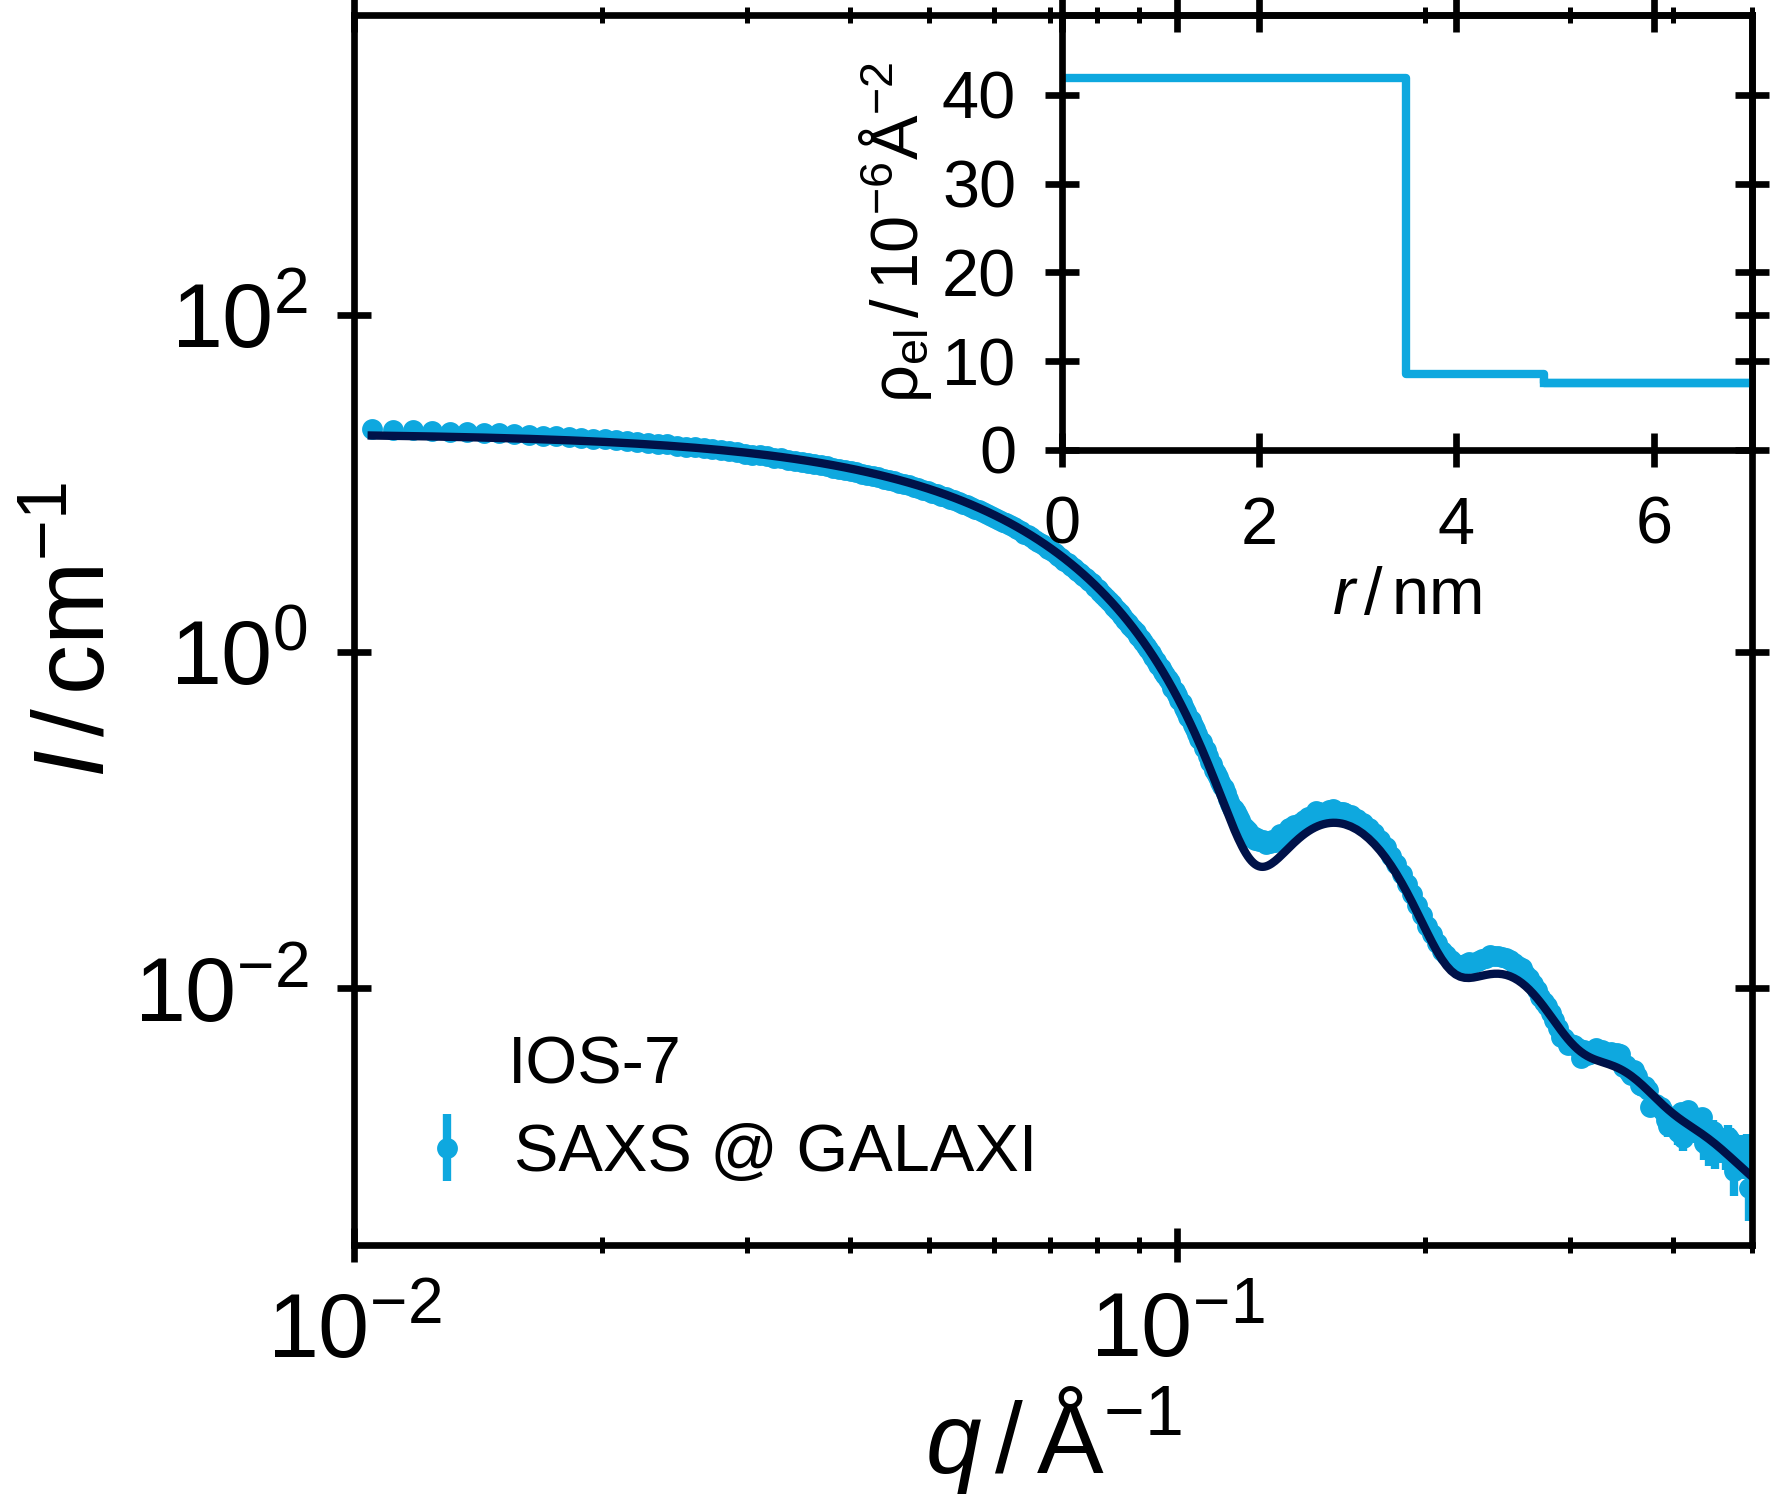
\includegraphics{looselyPackedNP_SAS_IOS-7_SAXS}
      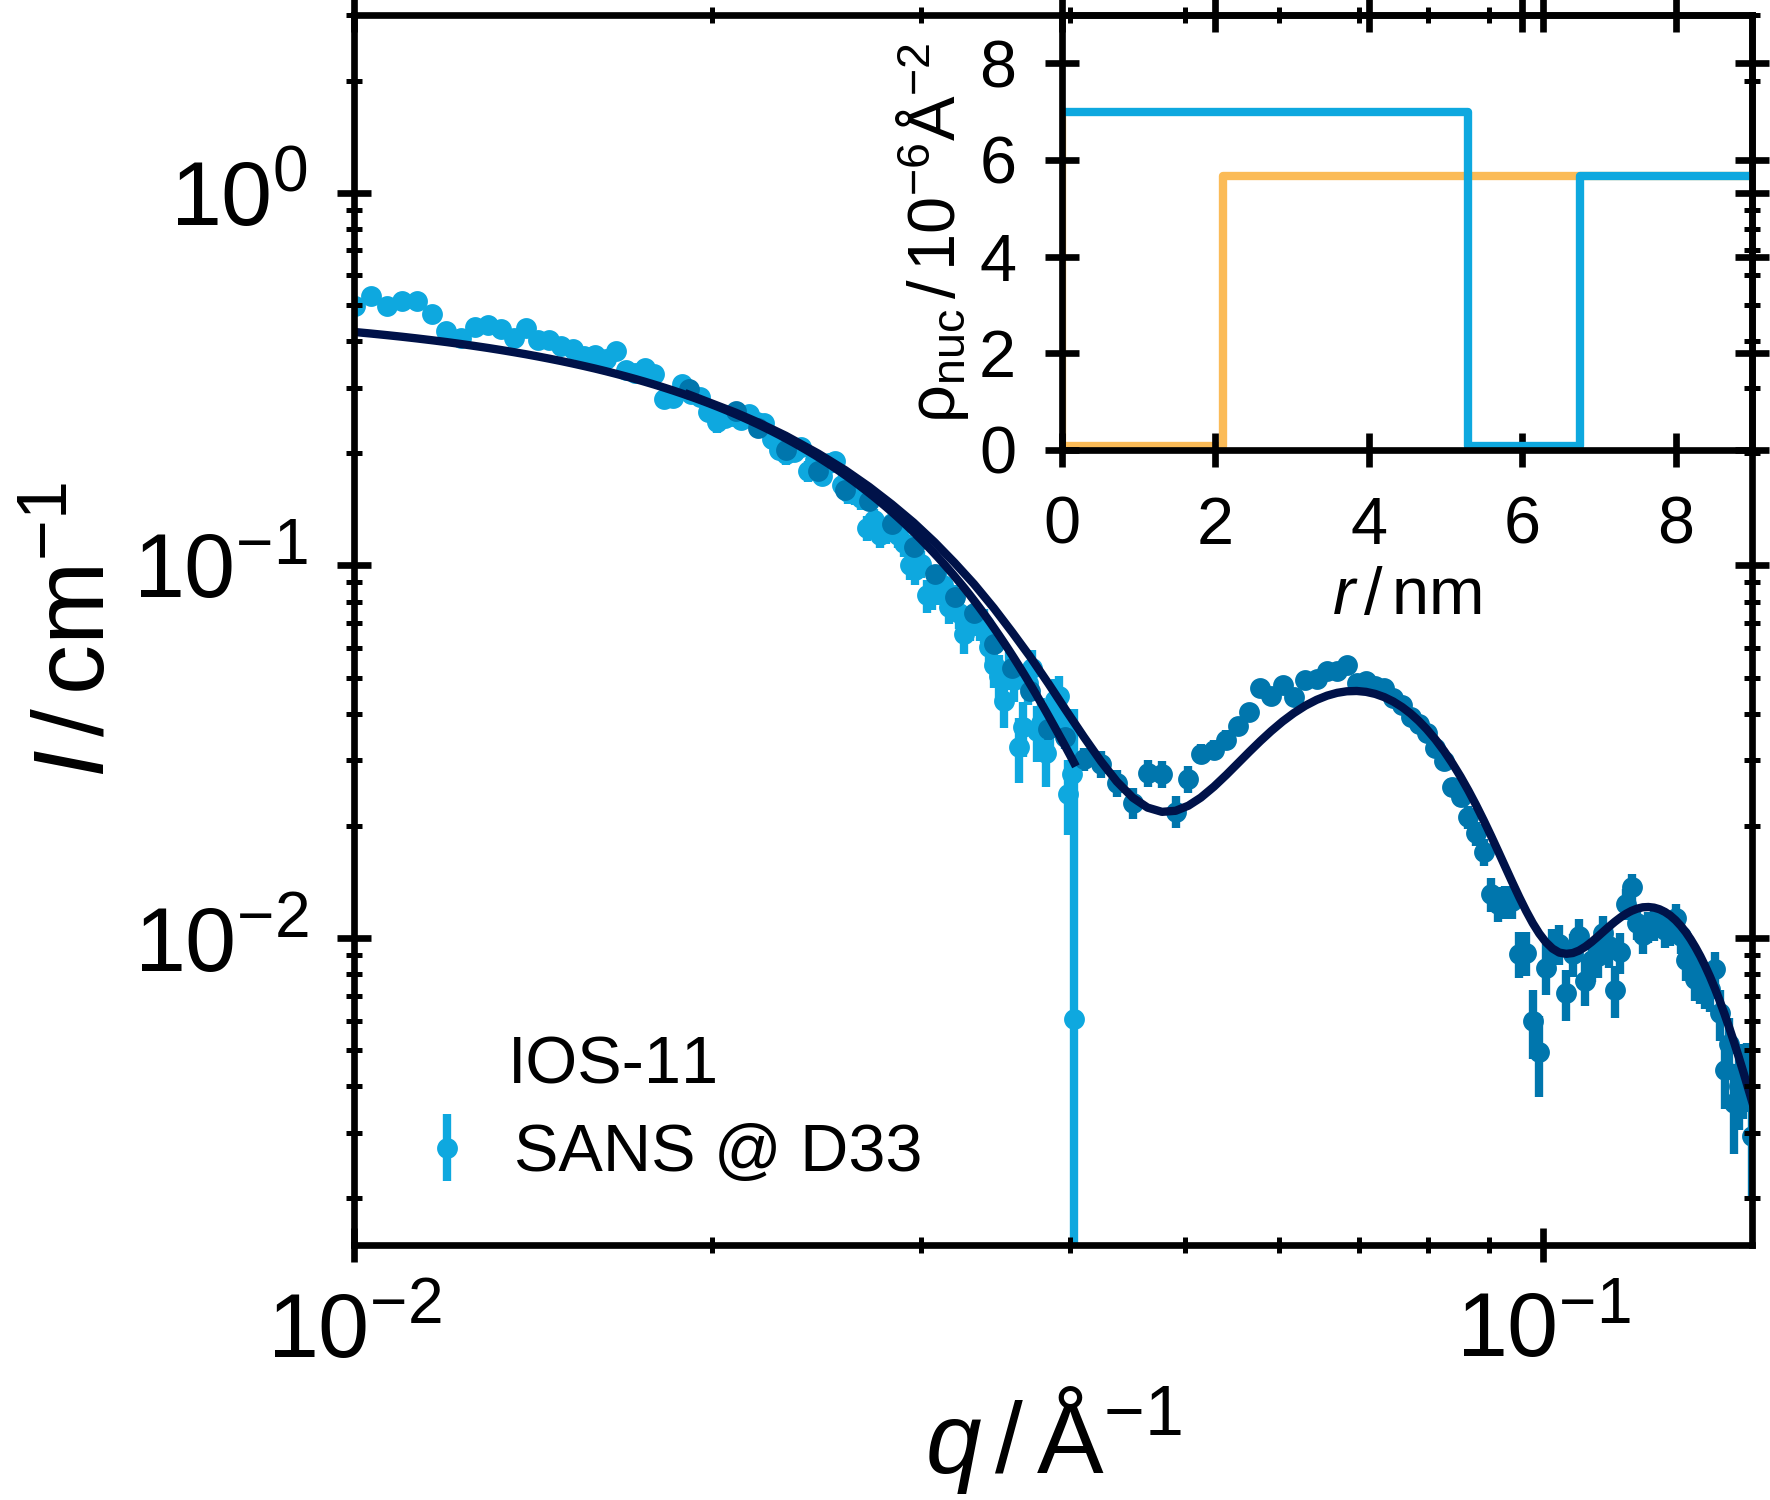
\includegraphics{looselyPackedNP_SAS_IOS-11_SANS}
      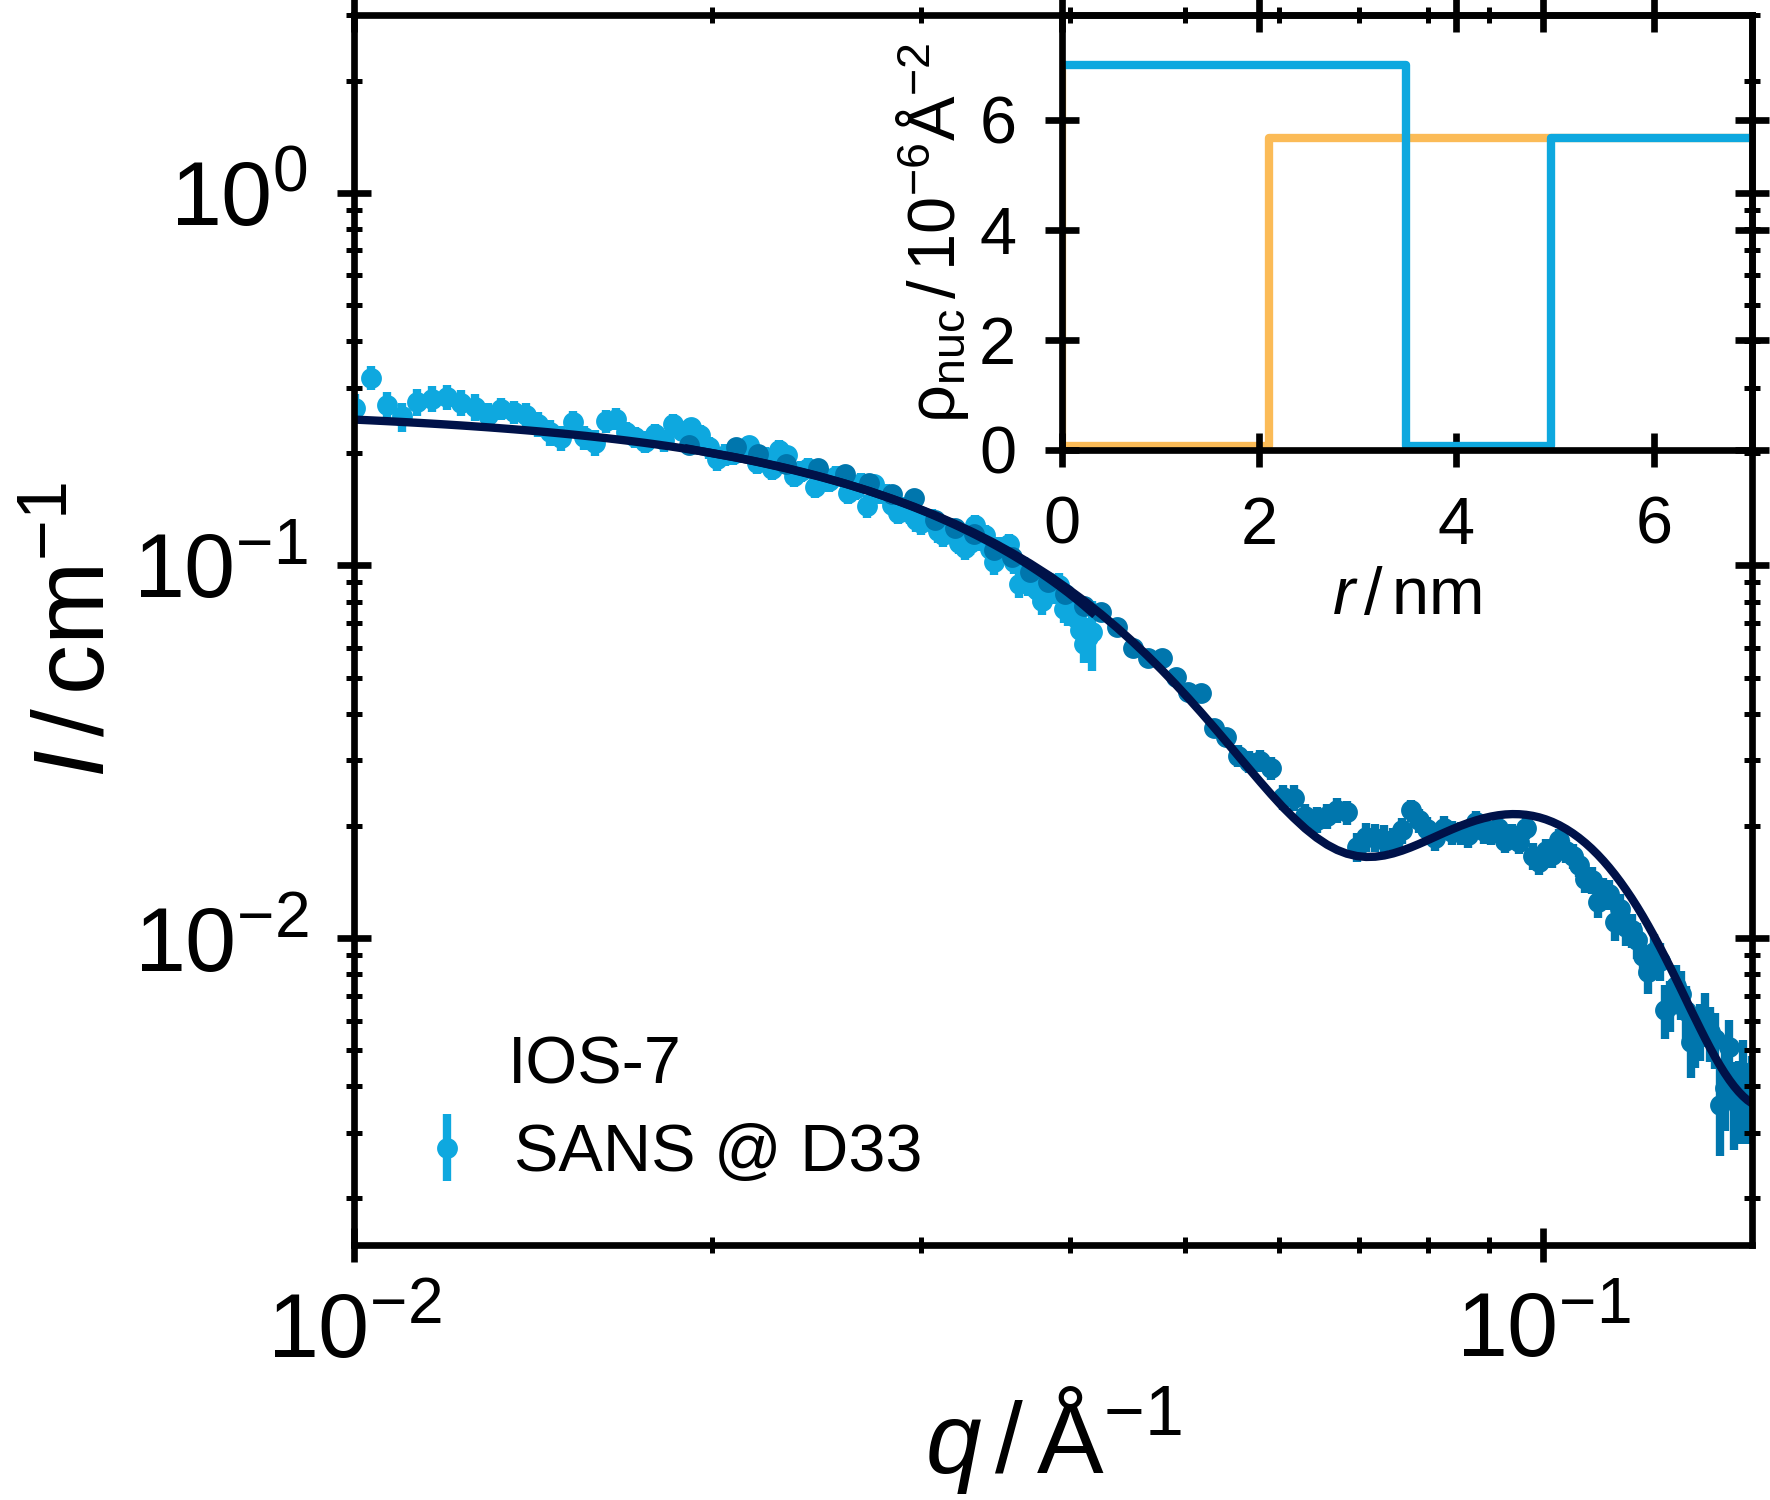
\includegraphics{looselyPackedNP_SAS_IOS-7_SANS}
      \caption{\label{fig:looselyPackedNP:nanoparticle:sas}Small-angle X-ray (upper) and neutron (lower) scattering for IOS-11 (left) and IOS-7 (right). The X-ray and neutron data sets are fitted to a spherical core-shell-surfactant form factor to estimate the average particle size, thickness of the two phases and the surfactant shell thickness, which are visible in the SLD profile insets. Additionally the particle size distribution is obtained and in the case of IOS-7 two modes are needed to describe the data properly (shown by two SLD profiles in the inset).}
    \end{figure}

    \begin{table}[!htbp]
      \centering
      \caption{\label{tab:looselyPackedNP:nanoparticle:sas}Parameters for the spherical core-shell model of IOS-11 and IOS-7.}
      \begin{tabular}{ c | l | l }
        \rule{0pt}{2ex} \textbf{SAXS}  & \textbf{IOS-11} & \textbf{IOS-7} \\
        \hline
        \rule{0pt}{2ex} $R_\mathrm{core} \, / \unit{nm}$                                    & $4.946(7)$           & $0$\\
        \rule{0pt}{2ex} $D_\mathrm{shell}\, / \unit{nm}$                                    & $0.456(7)$           & $3.540(2)$    \\
        \rule{0pt}{2ex} $\sigma_{(R+D)}\, / \unit{\%}$                                      & $5.45(2)$            & $7.52(6)$  \\
        \rule{0pt}{2ex} $\alpha \, / \unit{\%}$                                             &                      & $78(2)$\\
        \rule{0pt}{2ex} $R_{\mathrm{core},\, 2} \, / \unit{nm}$                             &                      & $0$\\
        \rule{0pt}{2ex} $D_{\mathrm{shell}, \, 2}\, / \unit{nm}$                            &                      & $0.680(4)$    \\
        \rule{0pt}{2ex} $\sigma_{(R_2 + D_2)}\, / \unit{\%}$                                &                      & $59.8(5)$   \\
        \rule{0pt}{2ex} $n \, / \unit{10^{-8} \angstrom^{-3}}$                              & $0.328(1)$           & $1.630(4)$\\
        \hline
        \rule{0pt}{2ex} $\rho_\textsf{w\"ustite} \, / \unit{10^{-6} \angstrom^{-2}}$        & \multicolumn{2}{c}{$52.07$}\\
        \rule{0pt}{2ex} $\rho_\mathrm{magnetite} \, / \unit{10^{-6} \angstrom^{-2}}$        & \multicolumn{2}{c}{$41.85$}\\
        \rule{0pt}{2ex} $\rho_\mathrm{oleic\, acid} \, / \unit{10^{-6} \angstrom^{-2}}$     & \multicolumn{2}{c}{$8.52$}\\
        \rule{0pt}{2ex} $\rho_\mathrm{cyclohexane} \, / \unit{10^{-6} \angstrom^{-2}}$      & \multicolumn{2}{c}{$7.55$}\\
        \hline
        \rule{0pt}{2ex} $c_m \, / \unit{mg\, mL^{-1}}$                                      & $12.1(1)$            & $3.5(1)$\\
        \hline
        \rule{0pt}{2ex} $\chi^2$                                                            & $25.9$               & $3.5$\\
        \hline
        \hline
        \rule{0pt}{2ex} \textbf{SANS} \\
        \hline
        \rule{0pt}{2ex} $R_\mathrm{core} \, / \unit{nm}$                                    & $3.8(1)$             & $0$\\
        \rule{0pt}{2ex} $D_\mathrm{shell}\, / \unit{nm}$                                    & $1.6(1)$             & $3.540$    \\
        \rule{0pt}{2ex} $R_{\mathrm{core},\, 2} \, / \unit{nm}$                             &                      & $0$\\
        \rule{0pt}{2ex} $D_{\mathrm{shell}, \, 2}\, / \unit{nm}$                            &                      & $0.680$    \\
        \rule{0pt}{2ex} $D_{\mathrm{oleic \, acid}, \, 2}\, / \unit{nm}$                    & $1.82(4)$            & $1.69(3)$    \\
        \rule{0pt}{2ex} $n \, / \unit{10^{-8} \angstrom^{-3}}$                              & $0.035(2)$           & $0.23(1)$\\
        \rule{0pt}{2ex} $I_\mathrm{bg} \, / \unit{cm^{-1}}$                                 & $0.0021(3)$          & $0.002(1)$\\
        \hline
        \rule{0pt}{2ex} $\rho_\textsf{w\"ustite} \, / \unit{10^{-6} \angstrom^{-2}}$        & \multicolumn{2}{c}{$8.34$}\\
        \rule{0pt}{2ex} $\rho_\mathrm{magnetite} \, / \unit{10^{-6} \angstrom^{-2}}$        & \multicolumn{2}{c}{$7.00$}\\
        \rule{0pt}{2ex} $\rho_\mathrm{oleic \, acid} \, / \unit{10^{-6} \angstrom^{-2}}$    & \multicolumn{2}{c}{$0.078$}\\
        \rule{0pt}{2ex} $\rho_{\mathrm{toluene-}d8} \, / \unit{10^{-6} \angstrom^{-2}}$     & \multicolumn{2}{c}{$5.66$}\\
        \rule{0pt}{2ex} $\lambda^\mathrm{sans} \, / \unit{\unit{\angstrom}}$                & \multicolumn{2}{c}{$6.00$}\\
        \rule{0pt}{2ex} $\Delta \lambda / \lambda \, / \unit{\%}$                           & \multicolumn{2}{c}{$4.247$}\\
        \rule{0pt}{2ex} $\Delta \theta_\mathrm{8 m} \, / \unit{mrad}$                       & \multicolumn{2}{c}{$2.1$}\\
        \rule{0pt}{2ex} $\Delta \theta_\mathrm{2 m} \, / \unit{mrad}$                       & \multicolumn{2}{c}{$3.8$}\\
        \hline
        \rule{0pt}{2ex} $c_m \, / \unit{mg\, mL^{-1}}$                                      & $1.2(1)$            &  $0.49(2)$\\
        \hline
    \rule{0pt}{2ex} $\chi^2$                                                                & $2.2$         & $1.3$\\
        \hline
      \end{tabular}
    \end{table}

  \paragraphNewLine{Comparison of Particle Sizes obtained by SAS with TEM and XRD}
    The obtained sizes from SAS, TEM and XRD for IOS-11 and SAS, TEM for IOS-7 are given in \reftab{tab:looselyPackedNP:nanoparticle:comparisonSASXRDTEM}.
    For both IOS-11 and the mode of IOS-7 with smaller size distribution, the obtained diameter of the core-shell structures from SAS ($5.41 \unit{nm}$ and $3.54 \unit{nm}$) is in close agreement to the value observed in TEM ($5.48 \unit{nm}$ and $3.49 \unit{nm}$).
    The observed particle size distribution from SAS ($5.45 \unit{\%}$ and $7.52 \unit{\%}$) is in both cases smaller than the value obtained by counting over $200$ nanoparticles in TEM ($6.6 \unit{\%}$ and $11 \unit{\%}$).
    For the second more of IOS-7 a larger discrepancy is visible between the size, fraction and size distribution observed in SAS ($0.68 \unit{nm}$, $78 \unit{\%}$ and $59.8 \unit{\%}$) with the values observed in TEM ($3.1 \unit{nm}$, $30 \unit{\%}$ and $29 \unit{\%}$).

    The deviations of the size distributions between SAS and TEM can be understood by the better statistics obtained in SAS, where the beam averages the particle size over $\mathcal{O}(10^{12})$ particles instead of only $200$ in TEM, and therefore a better precision can be achieved.
    Furthermore, for the small particles in the second mode of IOS-7, the resolution and limited view from TEM is not sufficient to properly estimate their size, fraction and size distribution.

    Comparing XRD and SAXS, the shell thickness of IOS-11 is larger in XRD ($2.557 \unit{nm}$) than in both SAXS ($0.46 \unit{nm}$) and SANS ($1.6 \unit{nm}$).
    On the one hand, the shell thickness can be overestimated in XRD due to the core-shell structure of the nanoparticle and a partially coherent scattering between two sides of the nanoparticle.
    On the other hand, the XRD experiment was performed approximately three years after the SAS experiment.
    And possibly an extended oxidation may have proceeded for the particles in dispersion over the years.
    Both facts contribute as to why the shell thickness in XRD is observed to be significantly larger.

    \begin{table}[!htbp]
      \centering
      \caption{\label{tab:looselyPackedNP:nanoparticle:comparisonSASXRDTEM}Parameters for the spherical core-shell model of IOS-11 and IOS-7.}
      \begin{tabular}{ c | l | l | l | l}
        \rule{0pt}{2ex} & \textbf{TEM} & \textbf{XRD} & \textbf{SAXS} & \textbf{SANS} \\
        \hline
        \rule{0pt}{2ex} \textbf{IOS-11}\\
        \hline
        \rule{0pt}{2ex} $R_\mathrm{core} \, / \unit{nm}$            &               & $3.721(1)$  & $4.946(7)$ & $3.8(1)$\\
        \rule{0pt}{2ex} $D_\mathrm{shell}\, / \unit{nm}$            &               & $2.557(1)$  & $0.46(7)$  & $1.6(1)$ \\
        \rule{0pt}{2ex} $R+D             \, / \unit{nm}$            & $5.48(3)$     &             & \multicolumn{2}{c}{$5.41(7)$}\\
        \rule{0pt}{2ex} $\sigma_{(R+D)}  \, / \unit{\%}$            & $6.6(4)$      &             & \multicolumn{2}{c}{$5.45(2)$}\\
        \hline
        \rule{0pt}{2ex} \textbf{IOS-7}\\
        \hline
        \rule{0pt}{2ex} $R_\mathrm{core} \, / \unit{nm}$            &               &             & \multicolumn{2}{c}{$0$}\\
        \rule{0pt}{2ex} $D_\mathrm{shell}\, / \unit{nm}$            &               &             & \multicolumn{2}{c}{$3.540(2)$}\\
        \rule{0pt}{2ex} $R+D             \, / \unit{nm}$            & $3.49(3)$     &             & \multicolumn{2}{c}{$3.540(2)$}\\
        \rule{0pt}{2ex} $\sigma_{(R+D)}  \, / \unit{\%}$            & $11(1)$       &             & \multicolumn{2}{c}{$7.52(6)$}\\
        \rule{0pt}{2ex} $\alpha \, / \unit{\%}$                     & $30(10)$      &             & \multicolumn{2}{c}{$78(2)$}\\
        \rule{0pt}{2ex} $R_{\mathrm{core},\, 2} \, / \unit{nm}$     &               &             & \multicolumn{2}{c}{$0$}\\
        \rule{0pt}{2ex} $D_{\mathrm{shell}, \, 2}\, / \unit{nm}$    &               &             & \multicolumn{2}{c}{$0.680(4)$}\\
        \rule{0pt}{2ex} $R_2 + D_2       \, / \unit{nm}$            & $3.1(3)$      &             & \multicolumn{2}{c}{$0.680(4)$}\\
        \rule{0pt}{2ex} $\sigma_{(R_2 + D_2)}\, / \unit{\%}$        & $29(4)$       &             & \multicolumn{2}{c}{$59.8(5)$}\\
        \hline
      \end{tabular}
    \end{table}

  \paragraphNewLine{Magnetic Structure from SANSPOL}
    Fixing the result for SANS, the magnetic scattering length density profile can be determined from SANSPOL for both IOS-11 and IOS-7.
    \reffig{fig:looselyPackedNP:nanoparticle:sanspol} shows the SANSPOL data and the best fit obtained for assuming a magnetic core-shell form factor with the parameters listed in \reftab{tab:looselyPackedNP:nanoparticle:sanspol}.
    For the magnetite shell of IOS-11 a magnetization of $450 \unit{kA \, m^{-1}}$ is observed, whereas for the w\"ustite core a magnetization of $124\unit{kA \, m^{-1}}$ is given.
    The magnetization of IOS-7 is determined to $199 \unit{kA \, m^{-1}}$.

    The magnetization of magnetite can be compared to the bulk magnetization value of magnetite ($4 \mu_B$ per formula unit or $500 \unit{kA \, m^{-1}}$ \cite{Handley_2000_Moder}).
    The shell magnetization of IOS-11 is therefore close to the value of bulk, whereas IOS-7 that is completely oxidized, is only at half of that magnetization.
    Possibly, the antiphase boundaries take a stronger effect in the fully oxidized IOS-7 particles, where the defects are present across the complete volume, whereas for the only partly oxidized IOS-11 particles, still a near bulk like behaviour remains.
    The magnetization of the w\"ustite core in IOS-11 is then measured to be fairly lower in comparison to the magnetite shell and with a larger uncertainty ($124(17) \unit{kA \, m^{-1}}$).
    Bulk w\"ustite orders anti-ferromagneticly below $200 \unit{K}$ with a magnetic moment of $4 \mu_B$ per \ch{Fe^{2+}} \cite{Handley_2000_Moder}.
    The measurement of only a weak magnetism is therefore expected in this case.
    
    The volume weighted average of the magnetization of IOS-11 is given by $200(10) \unit{kA \, m^{-1}}$.
    Interestingly this is in a comparable order of magnitude as the magnetization obtained for the IOS-7 particles, where a core-shell structure did not yield a good agreement with the experimental data.

    \begin{figure}[!htbp]
      \centering
      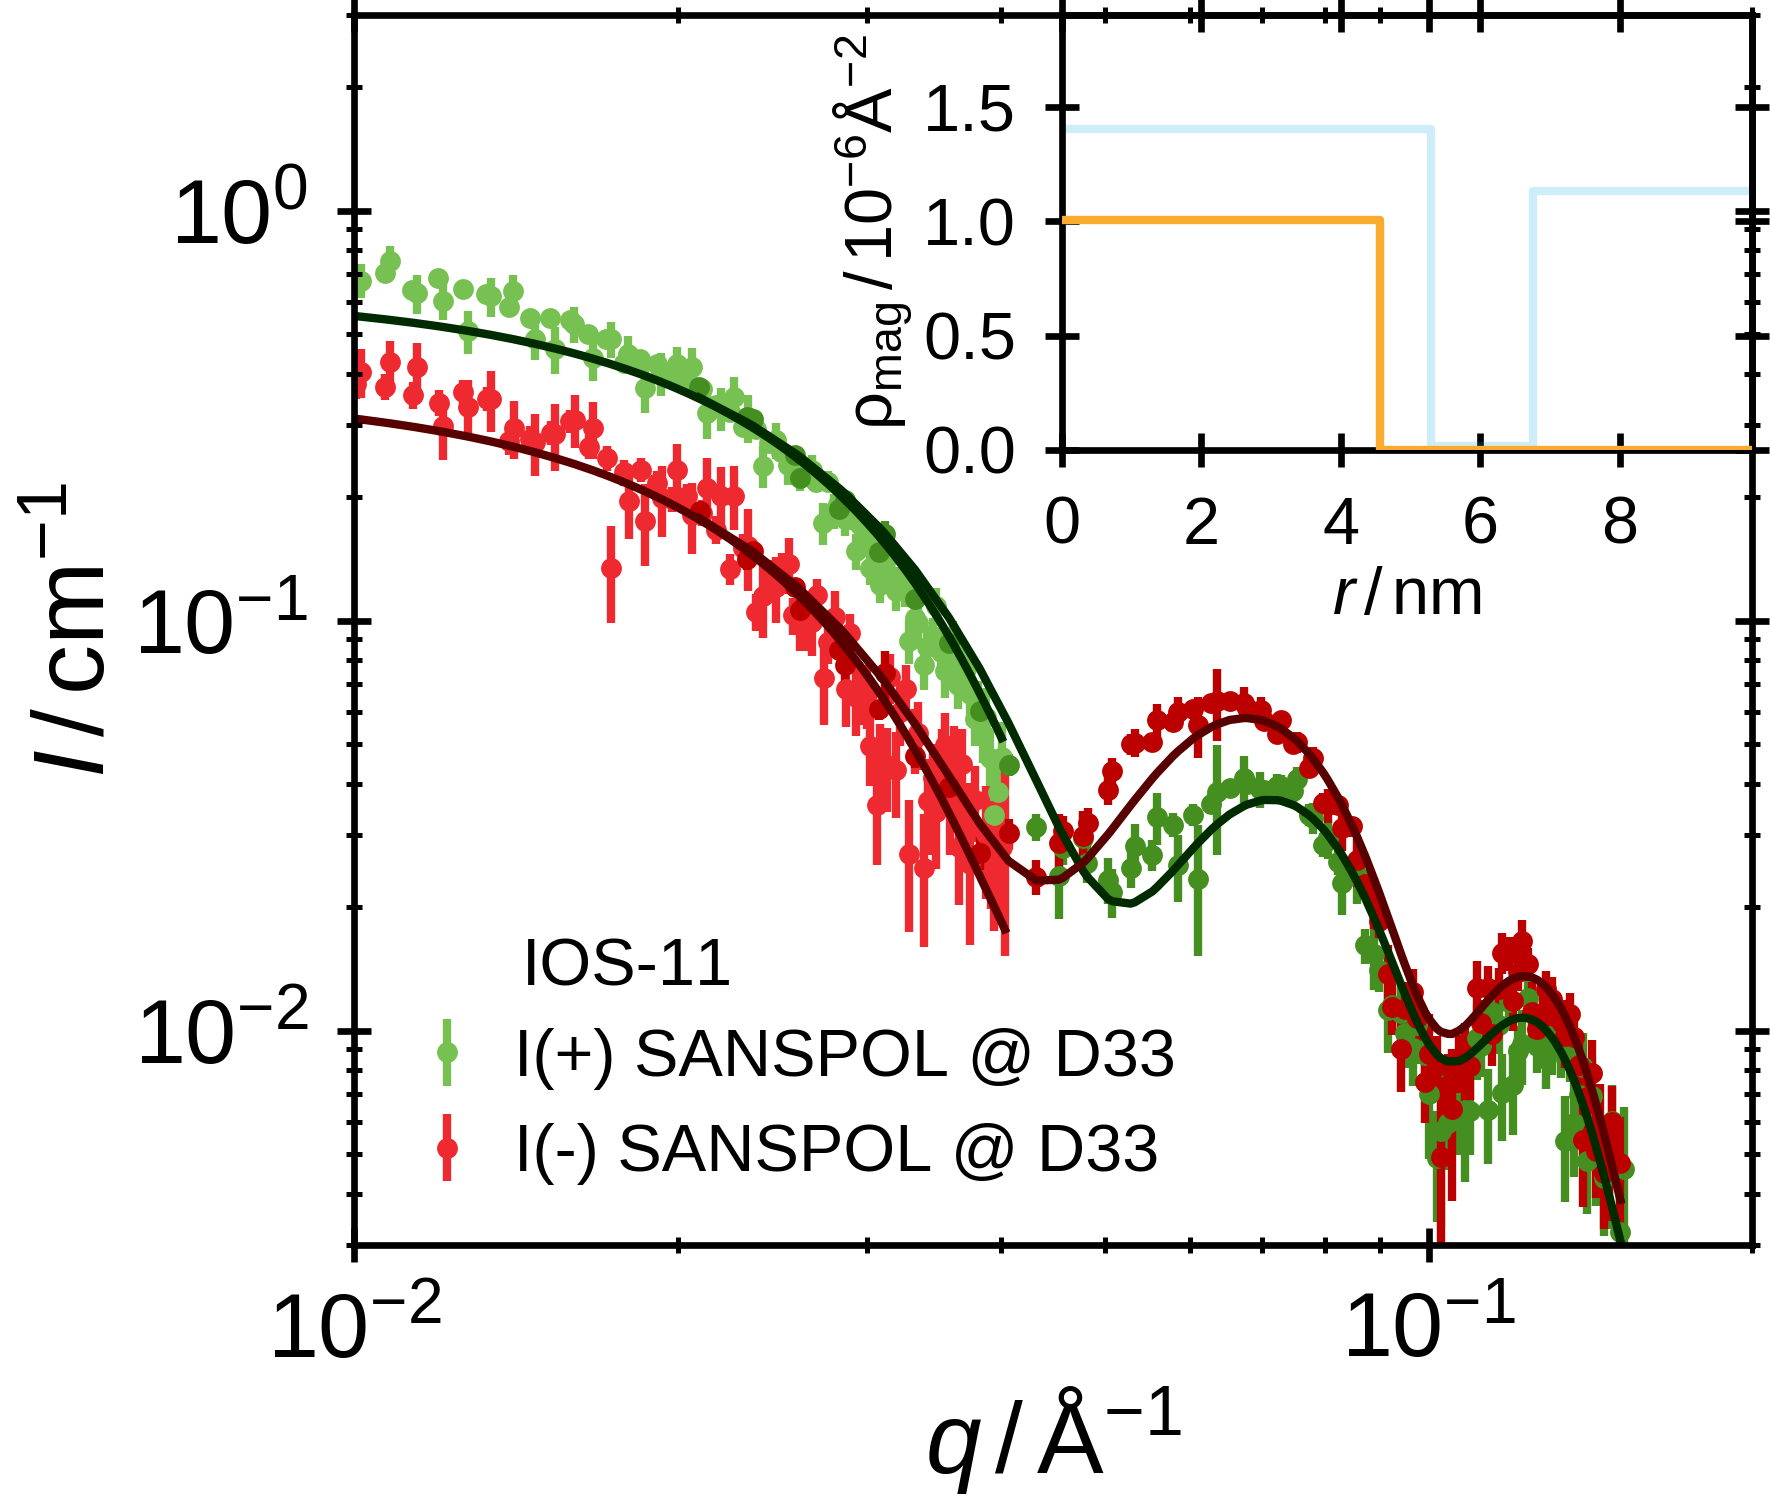
\includegraphics{looselyPackedNS_SAS_IOS-11_SANSPOL}
      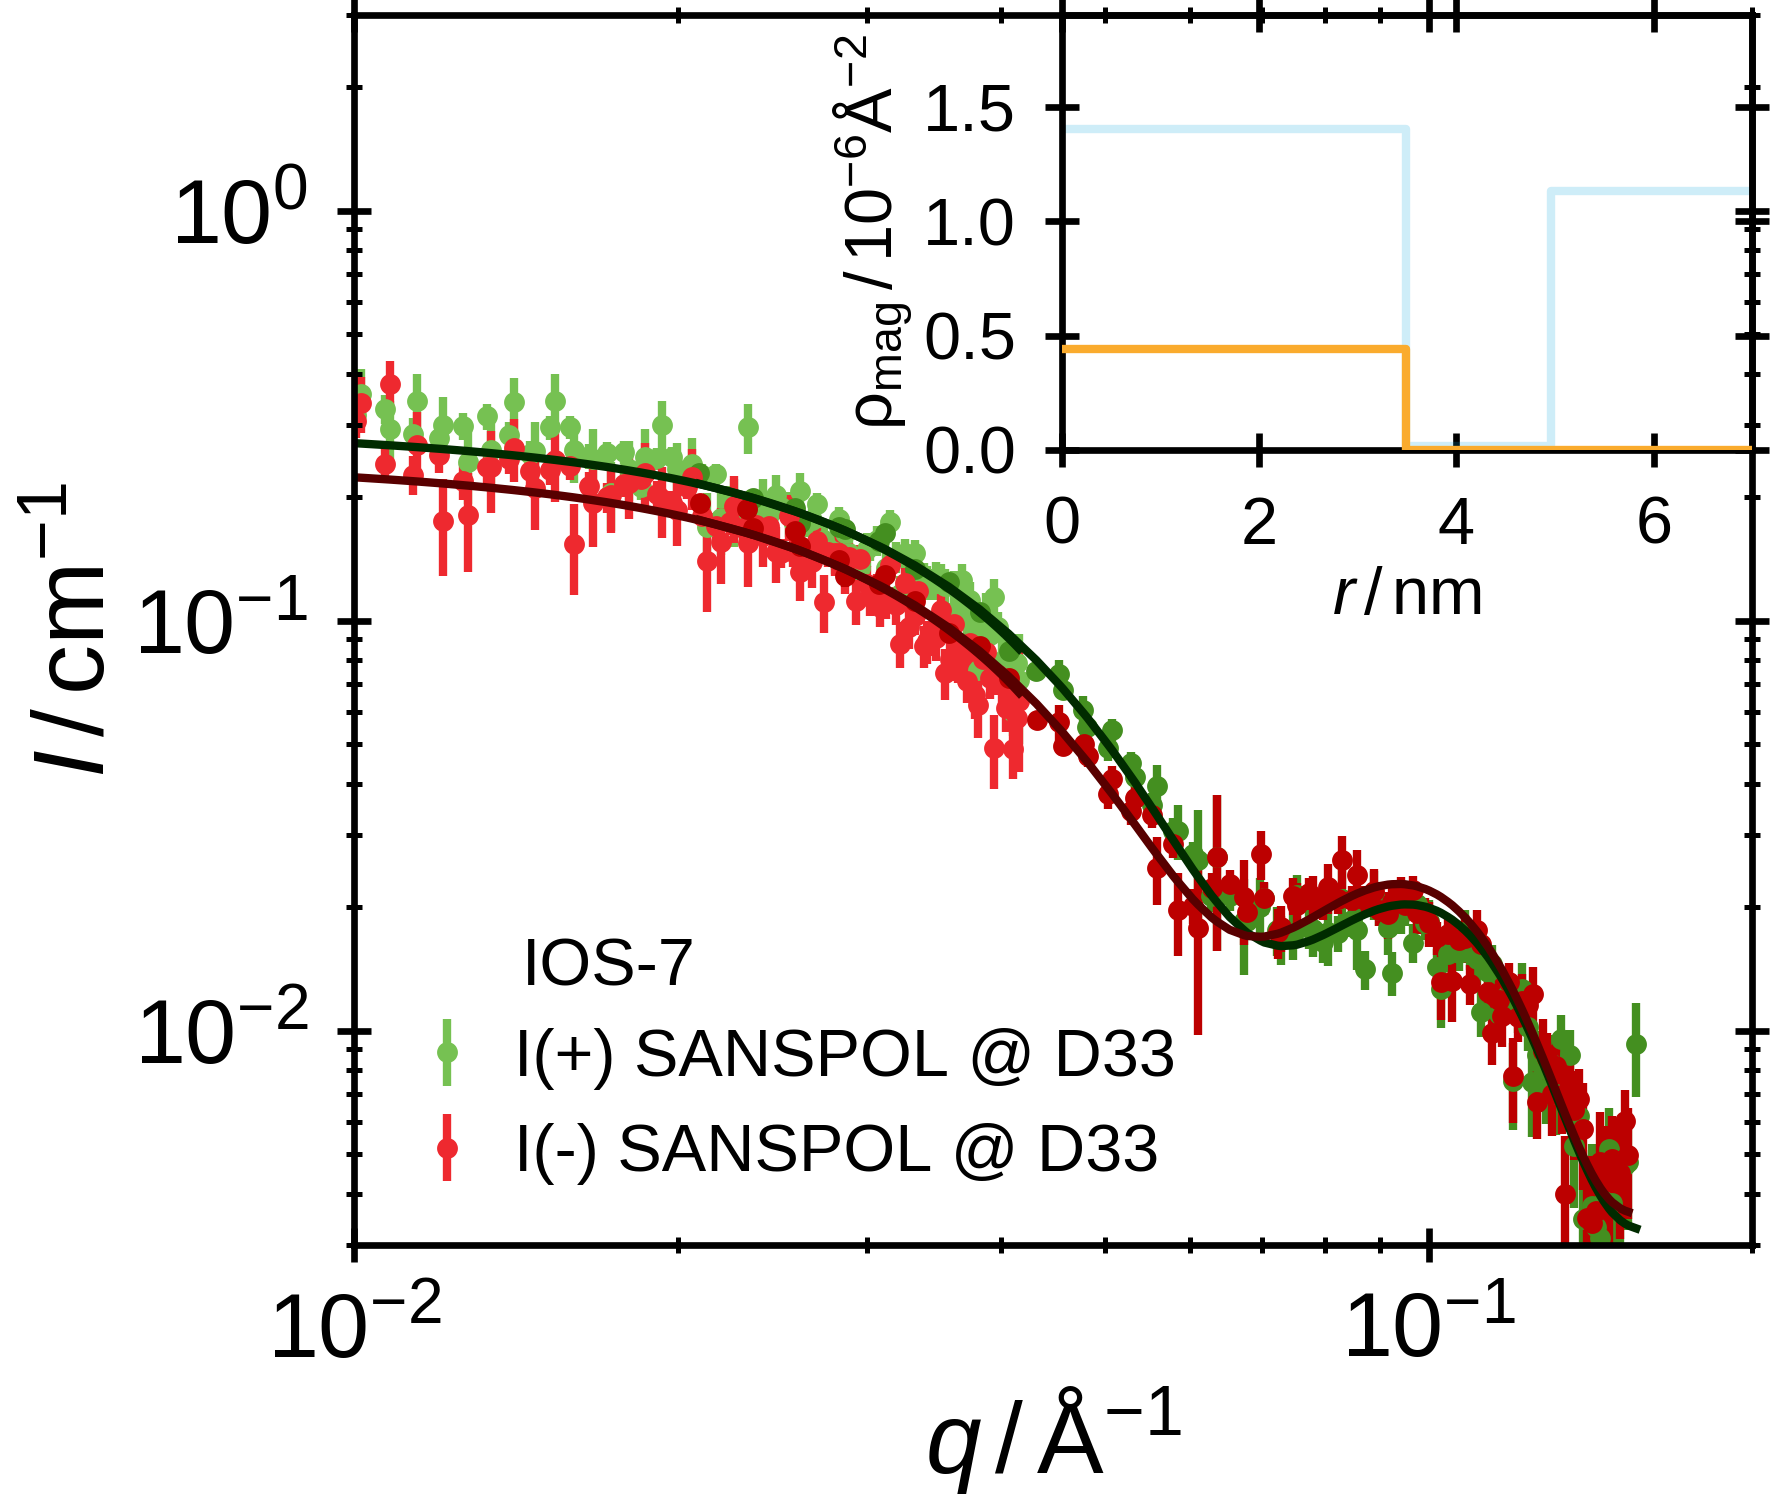
\includegraphics{looselyPackedNS_SAS_IOS-7_SANSPOL}
      \caption{\label{fig:looselyPackedNP:nanoparticle:sanspol}SANSPOL of IOS-11 (left) and IOS-7 (right).}
    \end{figure}

    \begin{table}[!htbp]
      \centering
      \caption{\label{tab:looselyPackedNP:nanoparticle:sanspol}Parameters for the spherical core-shell model of IOS-11 and IOS-7.}
      \begin{tabular}{ c | l | l }
        \rule{0pt}{2ex} \textbf{SANSPOL}  & \textbf{IOS-11} & \textbf{IOS-7} \\
        \hline
        \rule{0pt}{2ex} $\rho^\mathrm{mag}_\textsf{w\"ustite} \, / \unit{10^{-6} \angstrom^{-2}}$ & $0.36(5)$ & \\
        \rule{0pt}{2ex} $\rho^\mathrm{mag}_\mathrm{magnetite} \, / \unit{10^{-6} \angstrom^{-2}}$ & $1.32(4)$ & $0.58(4)$\\
        \hline
        \rule{0pt}{2ex} $M_\textsf{w\"ustite} \, / \unit{kA m^{-1}}$                              & $124(17)$ & \\
        \rule{0pt}{2ex} $M_\mathrm{magnetite} \, / \unit{kA m^{-1}}$                              & $453(14)$ & $199(14)$\\
        \hline
        \rule{0pt}{2ex} $\chi^2$                                                                  & $3.6$     & $1.7$\\
        \hline
      \end{tabular}
    \end{table}

\end{document}